\chapter{Представление результатов}
\section{Графики процента неактивной области}
    В разделе представления результатов были построены графики, отображающие процент наименее активных зон для различных каналов на каждом временном срезе. Эти графики позволяют визуализировать изменения в пространственно-временной динамике активности мозга.
    \begin{figure}[ht]
        \centering
        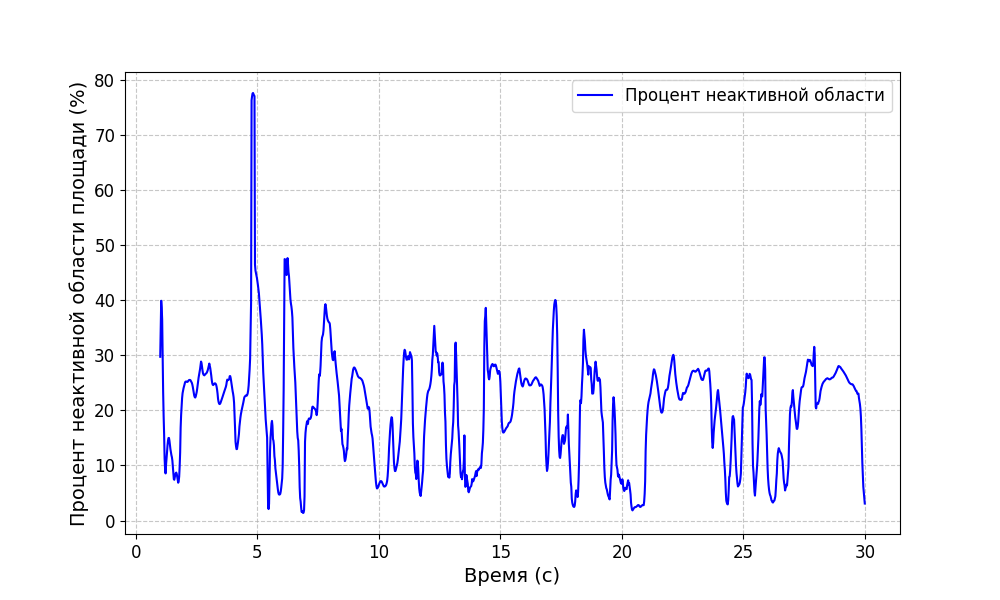
\includegraphics[width=1\textwidth]{images/delta_graphic.png}
        \caption{График, отображающий процент неактивной области для Delta-канала (0-4 Гц)}
        \label{fig:delta_graphic}
    \end{figure}
    \begin{figure}[ht]
        \centering
        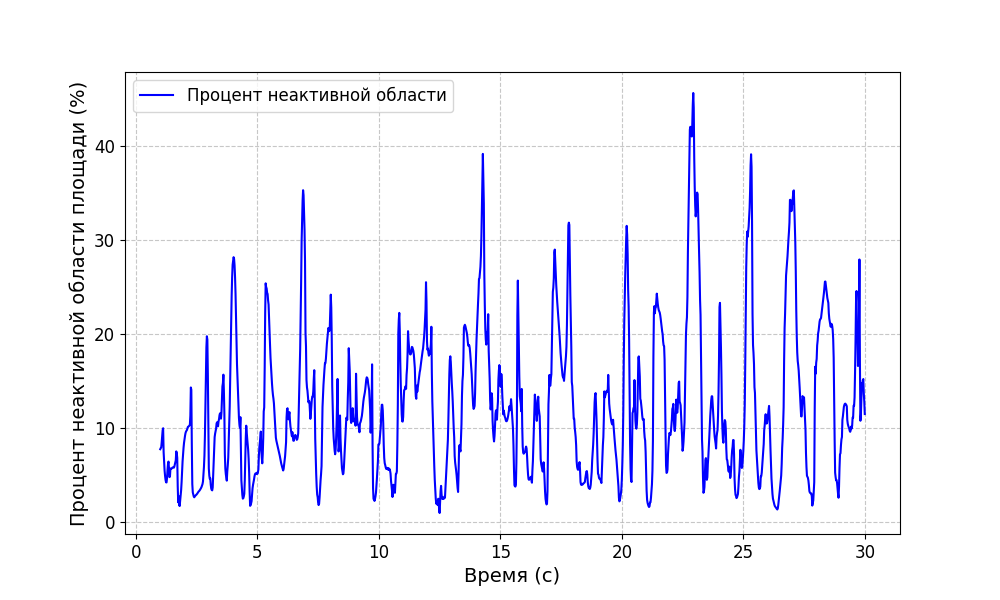
\includegraphics[width=1\textwidth]{images/theta_graphic.png}
        \caption{График, отображающий процент неактивной области для Theta-канала (4-8 Гц)}
        \label{fig:theta_graphic}
    \end{figure}
    \begin{figure}[ht]
        \centering
        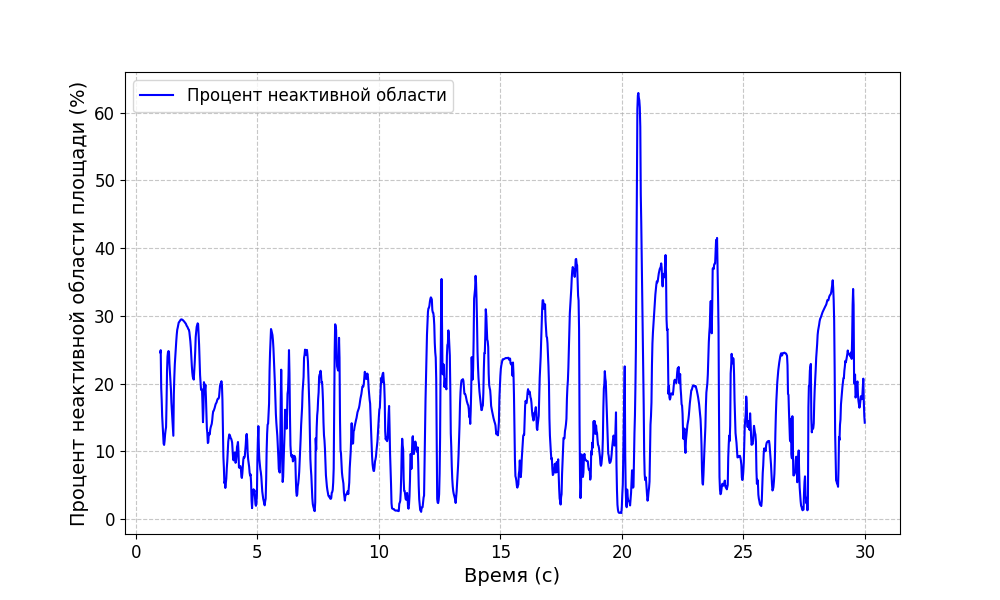
\includegraphics[width=1\textwidth]{images/alpha_graphic.png}
        \caption{График, отображающий процент неактивной области для Alpha-канала (8-12 Гц)}
        \label{fig:alpha_graphic}
    \end{figure}
    \begin{figure}[ht]
        \centering
        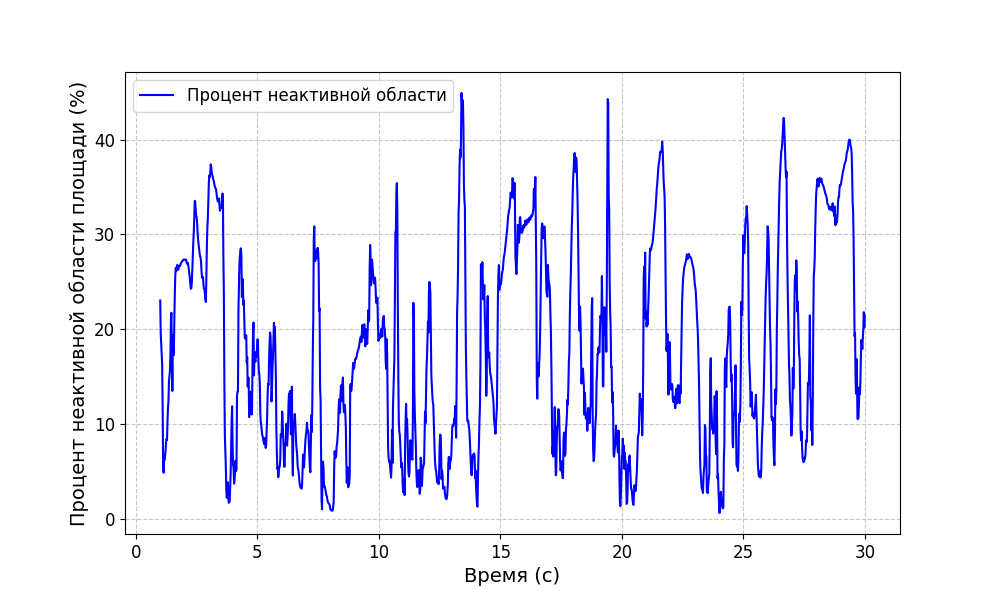
\includegraphics[width=1\textwidth]{images/beta_graphic.png}
        \caption{График, отображающий процент неактивной области для Beta-канала (12-30 Гц)}
        \label{fig:beta_graphic}
    \end{figure}
    \begin{figure}[ht]
        \centering
        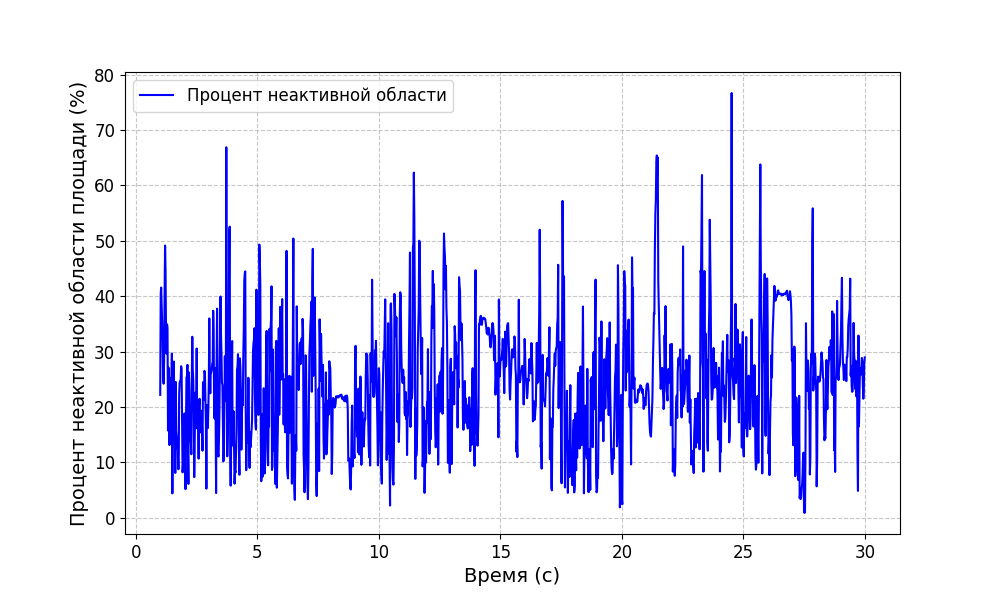
\includegraphics[width=1\textwidth]{images/gamma_graphic.png}
        \caption{График, отображающий процент неактивной области для Gamma-канала (30-45 Гц)}
        \label{fig:gamma_graphic}
    \end{figure}
    
\section{Среднее значение процента неактивной области}
Было вычислено среднее значение процента неактивной области для каждого канала на протяжении всего временного интервала. Полученные данные дают общее представление о характере активности для разных областей мозга, а также помогают выявить закономерности и аномалии в распределении активности в ходе эксперимента.

\begin{table}[ht]
\label{tab:t1}
\centering
\caption{Значение средних показателей процета неактивной области по частотным каналам}
\label{tab:table}
\begin{tabular}{|с|с|}
\hline
Канал    & Среднее значение процента неактивной зоны (\%) \\ \hline
Delta-канал (0-4 Гц)        & 20.11     \\
Theta-канал (4-8 Гц)        & 12.35     \\
Alpha-канал (8-12 Гц)       & 15.97     \\
Beta-канал (12-30 Гц)       & 17.90     \\
Gamma-канал (30-45 Гц)      & 24.01     \\ \hline
\end{tabular}
\end{table}

\section{Видеоролик с изменением топографических карт по времени}
Видео было создано посредством последовательного объединение бинарных изображений топографических карт. Каждое видео создано для отдельных каналов с соответсвующими названиями. Белыми областями представлены неактивные зоны.
\newline
Видео можно посмотреть по следующей \href{https://drive.google.com/drive/folders/1v-PtyjnEAI0c8PzsOospUVqq7BrCfBsq?usp=sharing}{ссылке:}
\newline
https://drive.google.com/drive/folders/1v-PtyjnEAI0c8PzsOospUVqq7BrCfBsq?u
sp=sharing

\endinput